\documentclass{standalone}
\usepackage{tikz}
\usetikzlibrary{matrix,chains,positioning,decorations.pathreplacing,arrows}
\usetikzlibrary{positioning, calc, chains}
\begin{document}


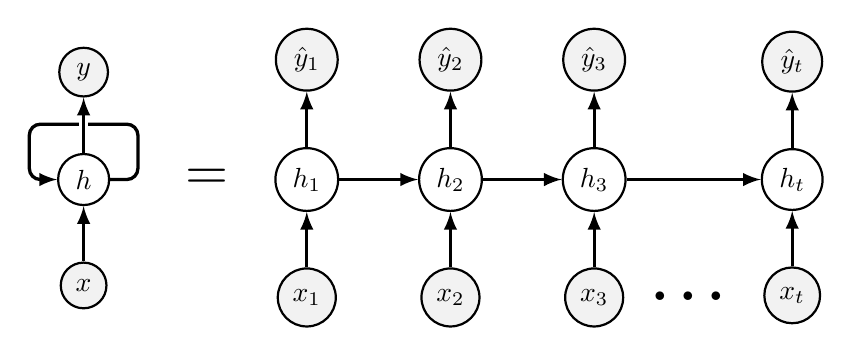
\begin{tikzpicture}[item/.style={circle,draw,thick,align=center},
itemc/.style={item,on chain,join}]
\begin{scope}[start chain=going right,nodes=itemc,every
join/.style={-latex,very thick},local bounding box=chain]
\path node (h1) {$h_1$} node (h2) {$h_2$} node (h3) {$h_3$} node[xshift=2em] (ht)
{$h_t$};
\end{scope}
\node[left=1em of chain,scale=2] (eq) {$=$};
\node[left=2em of eq,item] (AL) {$h$};
\path (AL.west) ++ (-1em,2em) coordinate (aux);
\draw[very thick,-latex,rounded corners] (AL.east) -| ++ (1em,2em) -- (aux) 
|- (AL.west);
\foreach \T in {1,2,3,t} 
{\draw[very thick,-latex] (h\T.north) -- ++ (0,2em)
	node[above,item,fill=gray!10] (y\T) {$\hat y_\T$};
	\draw[very thick,latex-] (h\T.south) -- ++ (0,-2em)
	node[below,item,fill=gray!10] (x\T) {$x_\T$};}
\draw[white,line width=0.8ex] (AL.north) -- ++ (0,1.9em);
\draw[very thick,-latex] (AL.north) -- ++ (0,2em)
node[above,item,fill=gray!10] {$y$};
\draw[very thick,latex-] (AL.south) -- ++ (0,-2em)
node[below,item,fill=gray!10] {$x$};
\path (x3) -- (xt) node[midway,scale=2,font=\bfseries] {\dots};
\end{tikzpicture}
\end{document}